%-------------------------------------------------------
\documentclass{beamer}
\usepackage{lmodern}
\usefonttheme[onlymath]{serif}
% \usetheme{beaver}
% \usetheme{Hannover}
% \usetheme{Singapore}
% \usetheme{CambridgeUS}
% \usetheme{Boadilla}
\usetheme{Madrid}
% \usecolortheme{beaver}
\colorlet{beamer@blendedblue}{green!35!black}
% \usetheme{Frankfurt}
% \usecolortheme{beaver}
% \setbeamertemplate{navigation symbols}{}

%\hypersetup{pdfpagemode=FullScreen}

\usepackage[mode=build]{standalone}
\usepackage[absolute,overlay]{textpos}
\usepackage[utf8]{inputenc}
\usepackage[spanish]{babel}
\usepackage{hyperref}
\usepackage{tikz}
\usepackage{graphicx}
\usepackage{booktabs}
\usepackage{caption}
\usepackage[rightcaption]{sidecap}
\usepackage{caption}
\usepackage{makecell}
% \usepackage{emoji}
% \graphicspath{{../03-outputs/figures/}}

\usepackage{apacite}
%\usepackage{natbib}
\usepackage{etoolbox}
\renewenvironment{APACrefURL}[1][]{}{}
\AtBeginEnvironment{APACrefURL}{\renewcommand{\url}[1]{}}
\renewcommand{\doiprefix}{doi:~\kern-1pt}

\bibliographystyle{apacite}

\title{Web scraping}
\subtitle{Para economistas}
\author{Alejandro Acosta León}

\date{\today}

\logo{
\includegraphics[width=2.5cm]{C:/Users/alejo/OneDrive - Universidad de Las Américas/Ico/economia-logo.png}
}


%-------------------------------------------------------
\begin{document}
\maketitle

\section{Introducción}

\begin{frame}
	\frametitle{Expectativas}
	\begin{alertblock}{ }
		\centering
		\textbf{¿Qué esperas aprender en este taller?}
	\end{alertblock}
	\centering
	Escríbanlo en el siguiente \href{https://jamboard.google.com/d/19WqnJKwaRLCvGGu4GEPRmnxqqNuRQeV6afe8qo44bLQ/edit?usp=sharing}{Jamboard}

\end{frame}


\begin{frame}
	\frametitle{Teoría}
	\underline{\textbf{Conceptos}}
	\begin{itemize}
		\item ¿Qué es web scraping?
		\item Introducción al web scraping y sus aplicaciones.
		\item Problemas éticos, legales y mal uso del web scraping.
		\item Alternativas al web scraping.
		\item Herramientas y librerías necesarias.
	\end{itemize}
	
	\underline{\textbf{Entorno}}
	\begin{itemize}
		\item Instalación de Python y librerías necesarias (requests, BeautifulSoup, pandas, selenium).
		\item Configuración del entorno de desarrollo (puede ser Jupyter Notebook, VSCode, etc.).
	\end{itemize}	
	
\end{frame}


\begin{frame}
	\frametitle{Práctica}
	\underline{\textbf{Nivel 1: data estructurada en HTML}}
	\begin{itemize}
		\item pandas
	\end{itemize}
	
	\underline{\textbf{Nivel 2: data semi-estructurada}}
	\begin{itemize}
		\item Inspección de elementos HTML.
		\item Extracción de datos con BeautifulSoup.
		\item Descarga de archivos.
	\end{itemize}

	\underline{\textbf{Nivel 3: data no estructurada que no usa HTML}}
	\begin{itemize}
		\item HTML y CSS.
		\item Inspección de elementos.
		\item Extracción de datos con BeautifulSoup.
	\end{itemize}
\end{frame}

\begin{frame}
	\frametitle{Algunos recursos importantes}
		\begin{itemize}
			\item Material del curso: \\
			\small{\url{https://github.com/alejo-acosta/favorita-powerbi/}}
			\item Descarga Power BI: \\
			\small{\url{https://powerbi.microsoft.com/en-us/downloads/}}
			\item Dataset original: \\
			\small{\url{https://www.kaggle.com/c/favorita-grocery-sales-forecasting/}}
			\item Documentación oficial de Power BI: \\
			\small{\url{https://docs.microsoft.com/en-us/power-bi/}}
			\item Lenguaje DAX (Power BI): \\
			\small{\url{https://docs.microsoft.com/en-us/dax/}}
			\item Lenguaje M (Power Query): \\
			\small{\url{https://docs.microsoft.com/en-us/powerquery-m/}}
		\end{itemize}
\end{frame}

\begin{frame}
	\frametitle{¿Qué es Power BI?}
	\begin{columns}
		\begin{column}{0.4\textwidth}
			\begin{itemize}
				\item Power BI suele definirse como: Herramienta corporativa de autoservicio para hacer business intelligence.
				\item BI son herramientas que nos permiten extraer, conectar y visualizar datos.
			\end{itemize}

		\end{column}
		\begin{column}{0.6\textwidth}
			\centering
			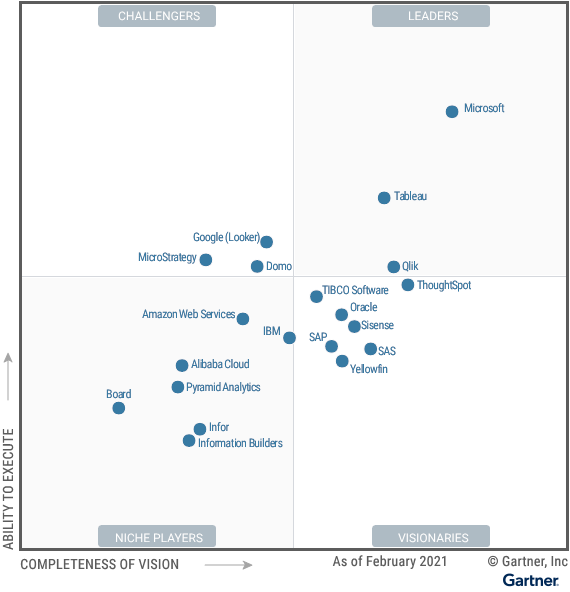
\includegraphics[scale=0.4]{quadrant.png} \\
			\tiny{\url{https://www.gartner.com/doc/reprints?id=1-24ZXJ0MU&ct=210107&st=sb}}
		\end{column}
	\end{columns}
	
\end{frame}

\begin{frame}
	\frametitle{¿Cuándo no usar Power BI?}
	\begin{alertblock}{ }
		\centering
		Power BI \textbf{no} es una herramienta de análisis o modelamiento de datos. \\
		Python, R, Stata, julia, etc. tienen una ventaja enorme en este campo. \\
		\textbf{El secreto es usar la herramienta adecuada para nuestro flujo de trabajo.}
	\end{alertblock}
	Por ejemplo:
	\begin{table}[!ht]
		\centering
		\resizebox{\textwidth}{!}{\begin{tabular}{|l|l|l|l|l|}
		\hline
		\makecell{Extracción y \\ manipulación datos} & \makecell{Análisis \\ Exploratorio} & \makecell{Gráficos y \\ reportes} & \makecell{Análisis \\  Estadístico} & Modelos \\ \hline
			\makecell{1.Python \\ 2.Excel \\ 3.Power BI \\ 4.Stata} & \makecell{1.Python \\ 2.Power BI \\ 3.Excel \\ 4.Stata} & \makecell{1.Python \\ 2.Power BI \\ 3.Excel} & \makecell{1.Python \\ 2.Stata} & \makecell{1.Stata \\ 2.R \\ 3.Python} \\ \hline
		\end{tabular}}
	\end{table}
\end{frame}


\begin{frame}
	\frametitle{Los lenguajes de Power BI}
	\begin{itemize}
		\item Power BI (al igual que Excel) tiene su propio "lenguaje de programación" llamado DAX. \\
		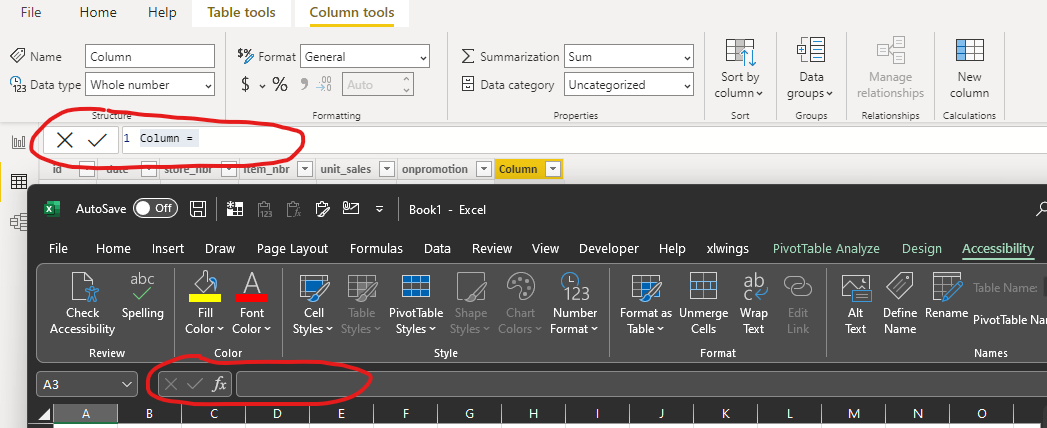
\includegraphics[scale=0.35]{excel.png} \\
		\item Sin embargo, también se utiliza otro lenguaje para extraer, transformar y cargar datos (ETL): M que es usado en Power Query.
	\end{itemize}

\end{frame}

\begin{frame}
	\frametitle{Dataset}
	\begin{itemize}
		\item Utilizaremos las ventas de Corporación la Favorita.
		\item Solo usaremos 1\% del total de la base. \\
	\end{itemize}	
	\small{\url{https://www.kaggle.com/c/favorita-grocery-sales-forecasting}}
	
\end{frame}

\begin{frame}
	\centering
	\frametitle<presentation>{Power BI}
	\framesubtitle{Parte II}
	En esta sesión revisaremos:
	\begin{itemize}
		\item Refuerzo de tablas 'dimensiones' y modelo relacional de datos.
		\item Datos long vs wide.
		\item Métricas.
		\item Merge y append.
		\begin{itemize}
			\item Funciones pivot y unpivot.
		\end{itemize}
		\item Series de tiempo descriptivas (no predictivas).
	\end{itemize}
  \end{frame}

  \begin{frame}
	\frametitle{Una pequeña motivación}
	\centering
	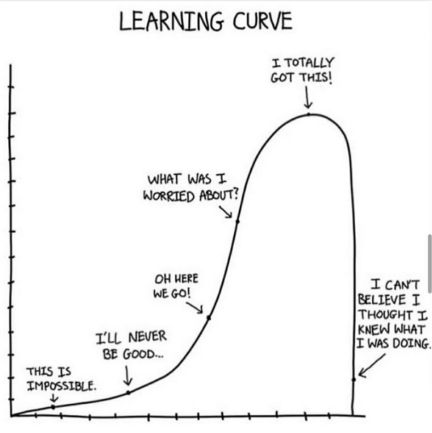
\includegraphics[scale=0.50]{learning-curve.png} \\
  \end{frame}
  
  \begin{frame}
	\centering
	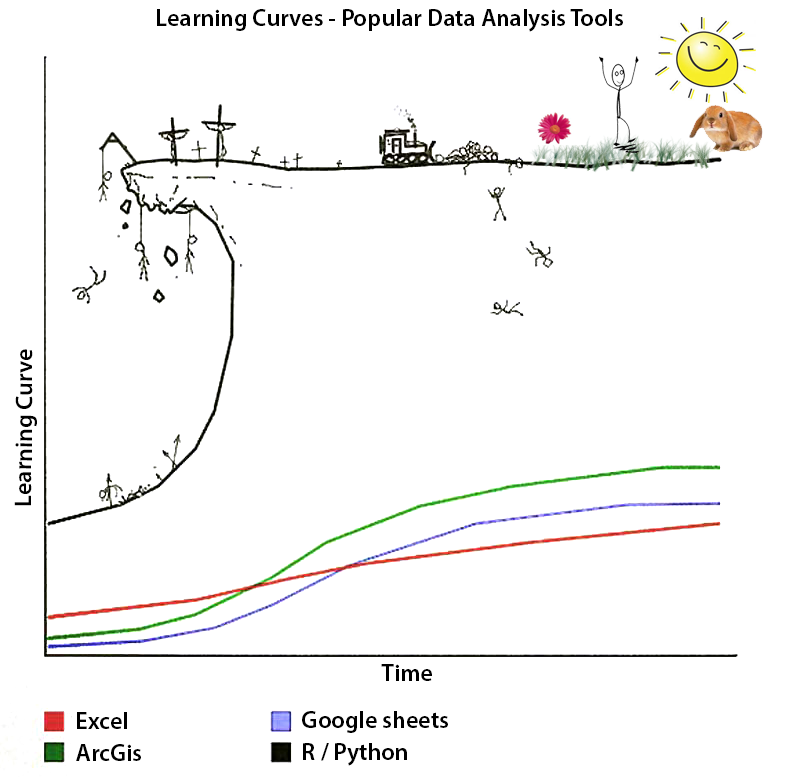
\includegraphics[scale=0.25]{learning_curve2.png} \\
  \end{frame}

  \end{document}